\section{Risultati}
Il risultato finale ottenuto dal progetto \emph{PathS} può essere consultato effettuando una richesta di \emph{routing} per una zona coperta dai campionamenti di test come quella presentata in figura \ref{fig:routing-3}.

In questa situazione tutte le operazioni di pre-processamento ed elaborazione dei dati si sintetizzano nel tipo di risposta che viene fornita. Nell'esempio presentato possiamo notare che:

\begin{itemize}
  \item i diversi tipi di calcolo si discostano nel risultato suggerendo percorsi diversi;
  \item i percorsi suggeriti hanno lunghezze totali analoghe, aumentando leggermente per rispettare la preferenza accordata (valutazione del rumore o della luminosità);
  \item il percorso più breve calcolato (in rosso) è praticamente coincidente con quello fornito dai servizi esterni (in blu);
  \item il percorso meno luminoso (indicato in grigio) cerca di evitare per quanto possibile le zone con campionamenti di luminosità dai valori alti;
  \item il percorso meno rumoroso (indicato in verde) non suggerisce il percorso più breve ma comprende tratti con campionamenti di rumore bassi;
\end{itemize}

\begin{figure}[ht]
  \centering
  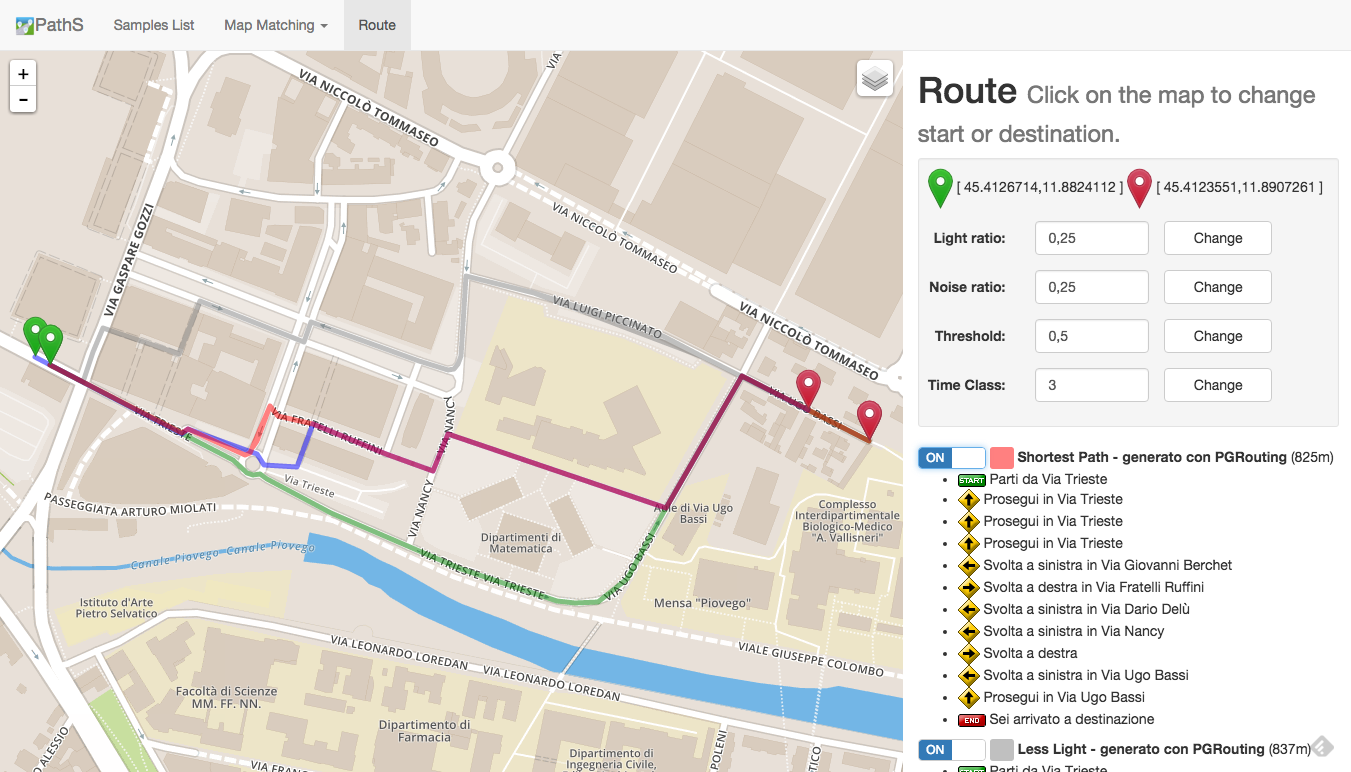
\includegraphics[width=\textwidth]{routing-3}
  \caption{\footnotesize{Esempio di richiesta di \emph{routing} per la classe temporale \texttt{3}.}}
  \label{fig:routing-3}
\end{figure}

Una conferma delle caratteristiche spazio-temporali della soluzione si può ottenere effettuando lo stesso tipo di interrogazione per una classe temporale diversa. Come si può vedere in figura \ref{fig:routing-4} i percorsi proposti sono diversi e tendono ad uniformarsi. Nella fascia oraria specificata infatti (dalle 17:59 alle 24:00) i campioni di luminosità non sono più molto influenti e quindi l'algoritmo propone un percorso molto più simile a quello più breve.

\begin{figure}[ht]
  \centering
  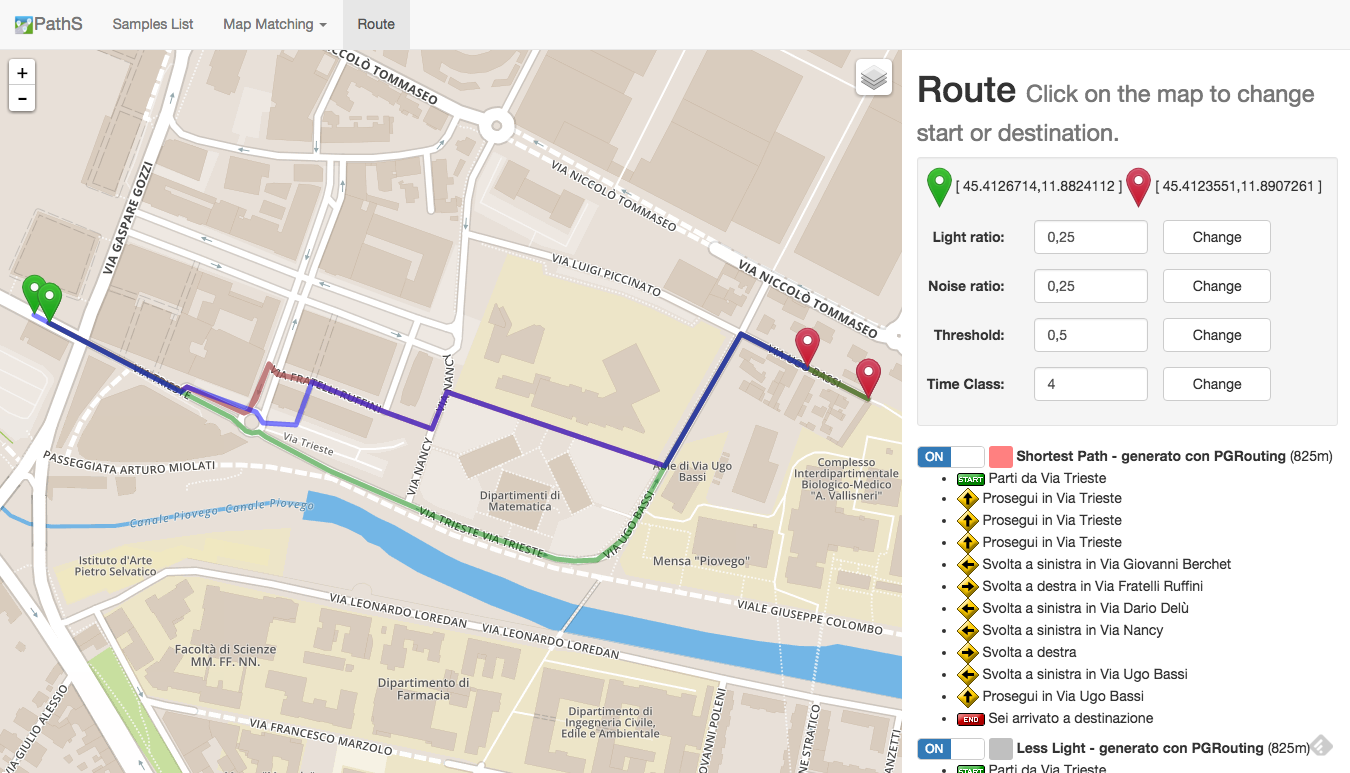
\includegraphics[width=\textwidth]{routing-4}
  \caption{\footnotesize{Esempio di richiesta di \emph{routing} per la classe temporale \texttt{4}.}}
  \label{fig:routing-4}
\end{figure}

Nei test effettuati il sistema ha presentato dei tempi di risposta accettabili per tutte le richieste di \emph{routing}. Per questi casi si ritiene che le prestazioni generali possano essere adeguate ad una interazione utente sia tramite browser che da terminale mobile. Per quanto riguarda le operazioni di processamento dei dati, pur essendo eseguite \emph{offline} e quindi non influenzando direttamente le attività degli utenti finali, potrebbero essere analizzate con maggiore dettaglio e probabilmente ottimizate ulteriormente.

Nello sviluppo di tutte le componenti si è cercato di seguire tutti i criteri di progettazione richiesti, utili ad un risultato facilmente modificabile ed estendibile.

\section{Miglioramenti ed Evoluzioni}
Già nella fase di sviluppo sono stati individuate alcune possibili aree di miglioramento, vengono presentate in seguito come spunto per possibili attività in futuro.
\subsubsection{Sistema di generazione di dati di test e procedura automatica di verifica}
Così come presentato nel \cite[capitolo~3.4]{mdme} può risultare utile l'adozione di un sistema di generazione di dati sinteci per le traiettorie. Questo approccio consentirebbe di accedere ad un'ampia base di dati controllati sulla quale valutare gli algoritmi sia in termini di \emph{performance} che in termini di correttezza e qualità dei risultati.

\subsubsection{Strategia di suddivisione segmenti}
Nell'implementazione attuale non viene applicato nessun intervento in termini di suddivisione dei segmenti. Questo semplifica le operazioni di assegnazione dei campioni e facilita la corrispondenza tra gli elementi salvati a sistema con quelli presenti nel servizio \emph{OpenStreetMap}. In alcuni casi limite tuttavia i segmenti forniti dalla cartografia possono risultare troppo estesi, in particolare se si presentano misurazioni con valori molto diversi. Un possibile miglioramento può riguardare quindi la procedura di analisi dei campioni introducendo l'operazione di suddivisione in sotto-segmenti per le situazioni in cui può migliorare la qualità dei dati a sistema.

\subsubsection{Algoritmi di map-matching}
Le attività del progetto si sono focalizzate nell'implementazione di un singolo algoritmo di \emph{Map matching} allo scopo di ottenere una prima soluzione funzionante. Può essere interessante riprendere l'analisi sulle alternative presenti in letteratura e implementare degli algoritmi alternativi. L'applicazione degli algoritmi ad un sistema automatico di generazione dei dati e di test potrebbe quindi portare ad una comparativa tra le varie soluzioni e ad una valutazione su quale sia l'implementazione che meglio si adatta al contesto e alla natura dei campioni raccolti.

\subsubsection{Algoritmi di routing}
Un ragionamento analogo al precedente può essere applicato alla selezione ed implementazione degli algoritmi di \emph{routing}. 

In una fase del progetto si è pensato di implementare questa componente da zero, applicando una soluzione di programmazione dinamica per \emph{Shortest Path Problem with Resource Constraints} (\emph{SPPRC}), sulla base dei lavori \cite[Desrochers~e~Soumis]{labelling} e successivi \cite[capitolo~4.4]{spprc}. 

Per difficoltà implementative, si è poi optato per la soluzione tramite l'utilizzo della libreria \emph{PGRouting}. La realizzazione di alcune alternative, possibilmente basate su algoritmi diversi, anche in questo caso potrebbe portare alle selezione di un prodotto che presenti caratteristiche migliori in termini di qualità dei risultati forniti o di complessità.

\subsubsection{Altri servizi}
I servizi offerti da \emph{PathS} potrebbero non riguardare solo le interrogazioni relative al \emph{routing}. I dati raccolti e il relativo processamento potrebbe essere una base di partenza per altri tipi di analisi, ad esempio uno studio sulle zone più frequentate nei diversi momenti della giornata o sui flussi più probabili. Analogamente si potrebbero sviluppare applicazioni del tipo ``\emph{get-together}'' che favoriscono l'incontro tra gli utenti e lo scambio di informazioni in chiave \emph{social}.
